\documentclass[12pt]{article}
%\documentstyle[12pt]{article}
%\usepackage{html}
\textwidth 6.5in
\topmargin -0.in
\textheight 8 in
\oddsidemargin -0.in
\evensidemargin -0.in
%\usepackage{graphics}  
\usepackage{graphicx}  
\begin{document}

\begin{center}
{\huge {\bf Handout 1: Review} }
\end{center}

\begin{itemize}

\item {\bf Basic Circuit Variables}
  \begin{itemize}
    \item {\bf Voltage:}

      Voltage is an ''across variable'' as it measures the difference between two electrical
      potentials at two points. When a reference point is used (e.g., the ''ground''), the
      voltage at a certain point is defined as the potential difference between this point
      and the reference point.

    \item {\bf Current:}

      Current is a ''through variable'' as it measures the amount of electrical charge that
      flow through a pass per unit time.

  \end{itemize}


\item {\bf Basic Elements}

  \begin{itemize}
  \item {\bf Resistor:}

    \[ V=RI,\;\;\;I=\frac{V}{R},\;\;\;R=\frac{V}{I} \]

  \item {\bf Capacitor:}

    \[ V=\frac{Q}{C}, \;\;\;i(t)=C\frac{d}{dt} v(t),\;\;\;
    v(t)=\frac{1}{C}\int_{-\infty}^t i(\tau) d\tau \]

  \item {\bf Inductor:}

    \[ V=\frac{W}{Q},\;\;\;\;\;v(t)=\frac{d}{dt} \psi(t)=L\frac{d}{dt} i(t),\;\;\;
    i(t)=\frac{1}{L}\int_{-\infty}^t v(\tau) d\tau \]

  \end{itemize}

\item {\bf Series and Parallel Connections}

  \begin{itemize}
  \item {\bf Series Connections:}
    \begin{figure}[hb]
      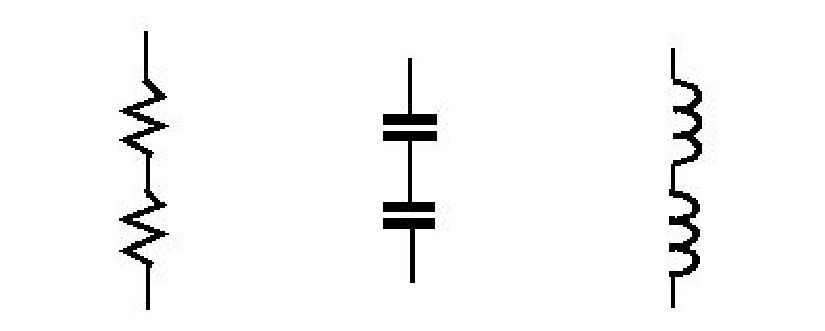
\includegraphics[scale=0.5]{figures/series_connections.eps}
    \end{figure}
	
    \[  R_{s}=R_1+\cdots+R_n=\sum_{i=1}^n R_i \]
    \[  L_{s}=L_1+\cdots+L_n=\sum_{i=1}^n L_i \]
    \[  \frac{1}{C_{s}}=\frac{1}{C_1}+\cdots+\frac{1}{C_n}
    =\sum_{i=1}^n \frac{1}{C_i},\;\;\;or\;\;\;
    C_{s}=\frac{1}{\sum_{i=1}^n \frac{1}{C_i}} \]
    If $n=2$,
    \[ C_s=\frac{1}{\frac{1}{C_1}+\frac{1}{C_2}}=\frac{C_1C_2}{C_1+C_2} \]

  \item {\bf Parallel Connections:}

    \begin{figure}
      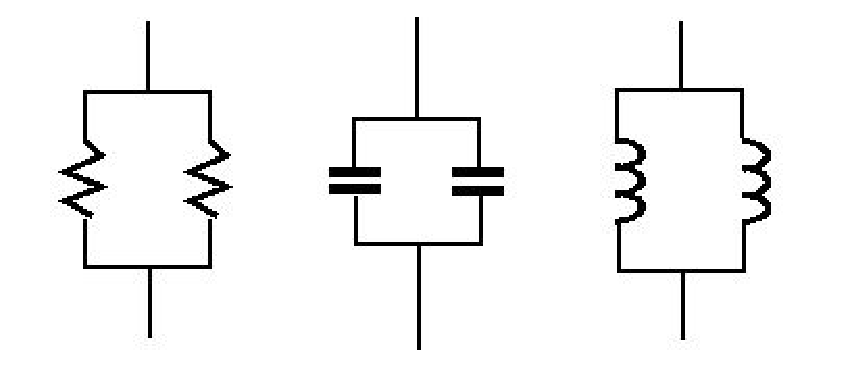
\includegraphics[scale=0.5]{figures/parallel_connections.eps}
    \end{figure}
    \[  \frac{1}{R_{p}}=\frac{1}{R_1}+\cdots+\frac{1}{R_n}
    =\sum_{i=1}^n \frac{1}{R_i},\;\;\;or\;\;\;
    R_{p}=\frac{1}{\sum_{i=1}^n \frac{1}{R_i}} \]
    If $n=2$,
    \[ R_p=\frac{1}{\frac{1}{R_1}+\frac{1}{R_2}}=\frac{R_1R_2}{R_1+R_2} \]
      
    \[  \frac{1}{L_{p}}=\frac{1}{L_1}+\cdots+\frac{1}{L_n}
    =\sum_{i=1}^n \frac{1}{L_i},\;\;\;or\;\;\;
    L_{p}=\frac{1}{\sum_{i=1}^n \frac{1}{L_i}} \]
    If $n=2$,
    \[ L_p=\frac{1}{\frac{1}{L_1}+\frac{1}{L_2}}=\frac{L_1L_2}{L_1+L_2} \]

    \[ C_{p}=C_1+C_2 \]
  \end{itemize}
  If $n=2$, we have:

  \begin{tabular}{c||c|c|c}\hline
    & \mbox{Resistor} & \mbox{Inductor} & \mbox{Capacitor} \\ \hline \hline
    v-i relation  & $v=R\;i$ & $v=L \;\frac{di}{dt}$  & $v=\frac{1}{C}\int i\;dt $ \\ \hline
    \mbox{Series}   & $R_s=R_1+R_2$ & $L_s=L_1+L_2$ & $C_s=C_1C_2/(C_1+C_2)$ \\ \hline
    \mbox{Parallel} & $R_p=R_1R_2/(R_1+R_2)$ & $L_p=L_1L_2/(L_1+L_2)$ & $C_p=C_1+C_2$ \\ \hline
  \end{tabular}

      {\bf Q:} Why are $R$ and $L$ similar to each other while $C$ is different?

      {\bf A:} Observe how $R$, $L$ and $C$ are related to voltage $v$ and current
      $i$ differently.
  
    \item {\bf Energy and Power}

      \[ V=\frac{W}{Q},\;\;\;W=VQ,\;\;\;P=\frac{dW}{dt}=V \frac{dQ}{dt}=VI=\frac{V^2}{R}=RI^2 \]

    \item {\bf Voltage/Current Dividers}

      \begin{figure}
	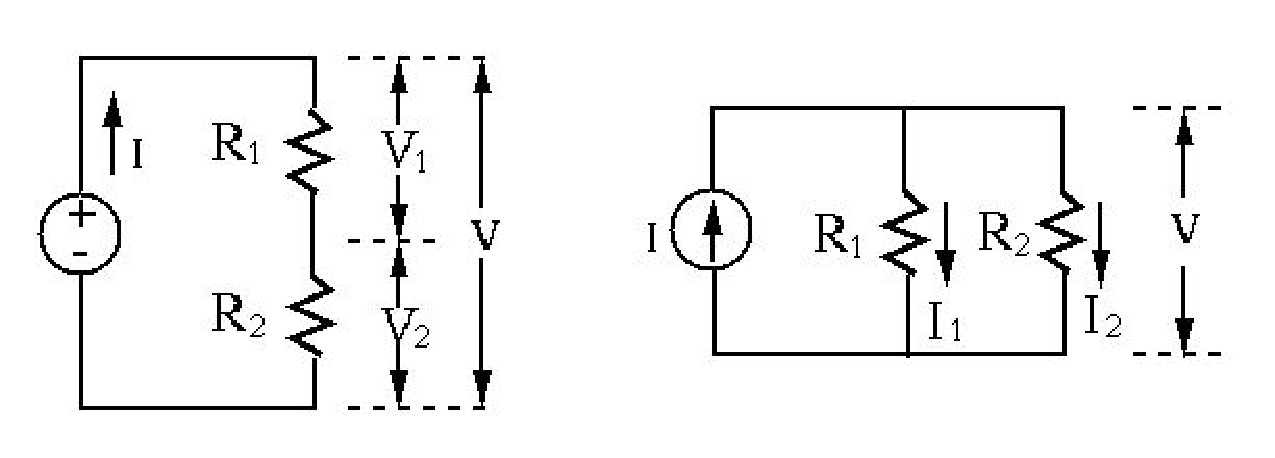
\includegraphics[scale=0.5]{figures/dividers.eps}
      \end{figure}
      \begin{itemize}
      \item {\bf Voltage Divider}
	\[ I=\frac{V}{R_1+R_2},\;\;\;\;V_1=IR_1=V\;\frac{R_1}{R_1+R_2},\;\;\;\;
	V_2=IR_2=V\;\frac{R_2}{R_1+R_2} \]
	Voltage across $R$ is proportional to its {\bf own} resistance.

	When there are more than two resistors in series, we simply have:
	\[ V_i=IR_i=V\;\frac{R_i}{\sum_j R_j} \]

      \item {\bf Current Divider}
	\[ V=I\frac{R_1R_2}{R_1+R_2},\;\;\;I_1=\frac{V}{R_1}=I\frac{R_2}{R_1+R_2},
	\;\;\;\;I_2=\frac{V}{R_2}=I\frac{R_1}{R_1+R_2}  \]
	Current through $R$ is proportional to {\bf the other} resistance.

	When there are more than two resistors in parallel, we have:
	\[ V=I\frac{1}{\sum_j 1/R_j},\;\;\;I_i=\frac{V}{R_i}=I\frac{1/R_i}{\sum_j 1/R_j}
	=I\frac{G_i}{\sum_j G_j} \]
	where $G_i=1/R_i$ is the {\em conductance} of the ith resistor.

      \end{itemize}
      
      \newpage
    \item {\bf Kirchoff's Laws}
      
      \begin{figure}
	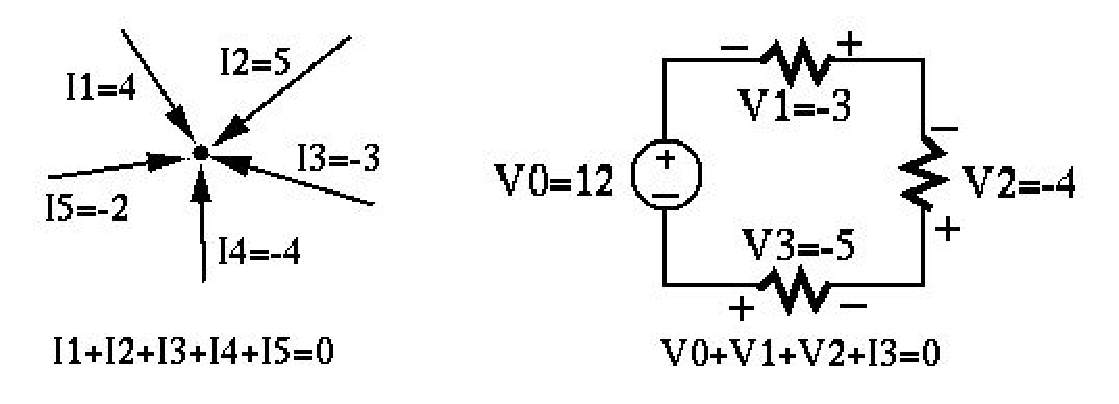
\includegraphics[scale=0.5]{figures/Kirchoff.eps}
      \end{figure}
      
      \begin{itemize} 
      \item {\bf KCL:} Due to conservation of electric charge, Kirchoff 
	current Law (KCL) states:
	
	The algebraic sum of all currents into a node is zero $\sum_k I_k =0$
	(Currents leaving the node take negative values.)
      \item {\bf KVL:} Due to conservation of electric energy, Kirchoff 
	voltage Law (KCL) states:

	The algebraic sum of voltage around a loop is zero $\sum_k V_k =0$
	(Voltages with opposite polarity take negative values.)

      \end{itemize}

    \item {\bf Reference Point or Ground}

      The voltage between any two nodes in a circuit is the difference between
      the potentials at the two nodes. However, a particular node in the
      circuit is usually chosen as the reference point, called the ground.
      The voltage at any node in the circuit is therefore defined as the 
      voltage between this node and the common ground.
      
\end{itemize}

\end{document}


	

	

